% Chapter 3: Algorithm description

\chapter{Descripción algorítmica} % Main chapter title

\label{Chapter3}

%-------------------------------------------------------------------------------
En este capítulo se describe el algoritmo metaheurístico utilizado, exponiendo todas sus características para la obtención de una solución al problema.

\section{Metaheurística GRASP\index{GRASP}}
\label{sec_metaGrasp}
El acrónimo \gls{GRASP} (Greedy Randomized Adaptative Search Procedure) o en castellano procedimiento de búsqueda voraz aleatorizado y adaptativo, fue introducido por primera vez por Feo y Resende en 1995 en su artículo con el mismo nombre \cite{grasp-feo-resende}.

Este algoritmo se basa en el multi-arranque, dónde cada uno de ellos es una iteración de un procedimiento que está constituido por dos partes bien diferenciadas. Por un lado, la fase constructiva, en la que se obtiene una solución de buena calidad, y por otro una fase de mejora, en la que, partiendo de la solución obtenida en la fase anterior, se intenta mejorar localmente \cite{libro-metaheuristicas}. 
En \cite{grasp-flightrecoveryproblem} \cite{grasp-parallel} \cite{grasp-weapon} \cite{grasp-empaquetado} \cite{grasp-ruta} \cite{grasp-vertex} se pueden encontrar diversos documentos en los que se tratan problemas aplicando la metaheurística \gls{GRASP}.

En el algoritmo \ref{alg:grasp} se muestra el pseudocódigo de la metaheurística \gls{GRASP} que se ha empleado para el desarrollo y obtención de una solución preliminar para este problema, y posteriormente, se muestra el algoritmo \ref{alg:bl}, con el cual se ha refinado esta solución para obtener una mejor.\\

\begin{algorithm}[H]
	\SetAlgoLined
	$ v \gets rnd( V ) $ \label{alg:grap:get_v} \\[0.2cm]
	$ S \gets \{ v \} $ \label{alg:grap:add_v_to_s} \\[0.2cm]
	$ CL \gets \{u \in V : (u, v) \in E\} $ \label{alg:grap:get_cl} \\[0.2cm]
	\While{$|CL| \not= 0$}{ \label{alg:grap:while} 
		$ c \gets CL$ \label{alg:grap:get_c} \\[0.2cm]
		$ \mathrm{g_{min}} \gets $ $ \smash{\displaystyle\min_{c \in CL}} \hspace{0.1cm} g(c) $ \label{alg:grap:get_gmax} \\[0.2cm]
		$ \mathrm{g_{max}} \gets $ $ \smash{\displaystyle\max_{c \in CL}} \hspace{0.1cm} g(c) $ \label{alg:grap:get_gmin} \\[0.2cm]
		$ \mu \gets  \mathrm{g_{max}} - \alpha ( \mathrm{g_{max}} - \mathrm{g_{min}} ) $ \label{alg:grap:get_mu} \\[0.2cm]
		$ RCL \gets \{ c \in CL : g(c) \geq \mu \}  $ \label{alg:grap:get_rcl} \\[0.2cm]
		$ u \gets rnd (RCL) $ \label{alg:grap:get_u} \\[0.2cm]
		$ S \gets S \cup \hspace{0.1cm} \{ u \}$ \label{alg:grap:add_u_to_s} \\[0.2cm]
		$ CL \gets CL \textbackslash \{ u \} \textbackslash \{ w : (u, w) \notin E \}$  \label{alg:grap:up_cl} \\[0.2cm]
	}
	\Return S \label{alg:grap:rt_s}
	\caption{Pseudocódigo algoritmo GRASP.}
	\label{alg:grasp}
\end{algorithm}

Dichos algoritmos se explicarán aplicados al problema tratado de la siguiente manera:

Teniendo un grafo $G=(V, E)$ donde $V$ son los vértices o nodos del grafo, y $E$ las aristas que unen estos nodos.\\
Se parte del paso \ref{alg:grap:get_v} del algoritmo \ref{alg:grasp}, donde se toma un vértice $v$ aleatorio de entre los vértices del grafo. En el paso \ref{alg:grap:add_v_to_s} el vértice $v$ se incluye en la solución $S$ ya que cumple con las restricciones del problema, descritas en la sección \ref{intro-problema}. A partir de $v$ se construye la lista de candidatos $CL$, como se indica en el paso \ref{alg:grap:get_cl}, definida como todos los nodos adyacentes a $v$ que forman parte de la lista de nodos del grafo de partida. A continuación, se toma un elemento de la lista de candidatos, paso \ref{alg:grap:get_c}, con el que se obtiene mediante una función voraz un listado de nodos. Esta función será determinada antes de iniciar el proceso e indicará si se deben obtener los nodos según su ratio o según el número de adyacentes al nodo tratado, será explicada con mayor detalle en la sección \ref{sec:faseConstructiva}. De este listado se escogen los valores de ratio máximo y mínimo de los nodos, descrito en los pasos \ref{alg:grap:get_gmax} y \ref{alg:grap:get_gmin}, y junto a $\alpha$ se obtiene el valor de $\mu$, mostrado en el paso \ref{alg:grap:get_mu}.

El valor de $\mu$ indica el umbral de la lista restringida de candidatos $RCL$. Esta lista se genera mediante la lista de candidatos $CL$ ordenada de mayor a menor valor y, como se muestra en la figura \ref{fig:rcl}, se toman los primeros valores hasta alcanzar el valor umbral, esa función está descrita  en el paso \ref{alg:grap:get_rcl}.

 \begin{figure}[H]
	\centering
	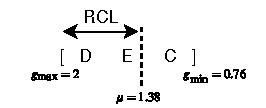
\includegraphics{Figures/rcl.pdf}
	\caption{Detalle de la lista restringida de candidatos (RCL).}
	\label{fig:rcl}
\end{figure}

Respecto al valor de $\alpha$, será configurado antes de este proceso y oscilará entre $0$ y $1$. Este valor va a indicar la cantidad de nodos que se incluirían en la $RCL$. Por un lado, un valor igual a $1$ supondría añadir el mejor candidato, convirtiendo el algoritmo en más voraz. Por el contrario, si se configura un valor de $0$, se estarían incluyendo más candidatos en el listado.

De la $RCL$ se elegirá, de manera aleatoria, un nodo $u$ como se muestra en el paso \ref{alg:grap:get_u}, se añadirá a la lista solución $S$, paso \ref{alg:grap:add_u_to_s} y será eliminado de la lista de candidatos junto con los nodos que no sean adyacentes a este, paso \ref{alg:grap:up_cl}.

Este procedimiento será repetido hasta que la lista de candidatos este vacía, obteniéndose en ese momento la lista $S$ final, que conformará la solución preliminar se devolverá en el paso \ref{alg:grap:rt_s} del algoritmo \ref{alg:grasp}. Esta solución será usada en la fase de mejora, explicada con detalle en la sección \ref{sec:faseBusqueda}, con el fin de optimizarla.

\subsection{Fase constructiva}
\label{sec:faseConstructiva}
En esta fase se ha usado el algoritmo \ref{alg:const_voraz} para definir la función constructiva. Esta es común a ambos constructivos y cada uno de ellos se especializa en como obtener el mejor nodo a incluir en el listado que será devuelto.\\

\begin{algorithm}[H]
	\SetAlgoLined
	$ S \gets \emptyset $ \label{alg:const_voraz:s_vacia} \\[0.2cm]
	$ Adyacentes \gets  SelecciónAdyacentes(nodo) $ \label{alg:const_voraz:get_adys} \\[0.2cm]
	\While{$|Adyacentes| \not= 0$}{
		$ candidato \gets buscarMejor(Adyacentes) $ \label{alg:const_voraz:get_mejor} \\[0.2cm]
		\If{formaClique(candidato)}{ \label{alg:const_voraz:cond_clique}
			$ Adyacentes \gets Adyacentes \cap SelecciónAdyacentes(candidato) $ \label{alg:const_voraz:up_adys} \\[0.2cm]
			$ S \gets S \cup \{candidato\} $ \label{alg:const_voraz:add_mejor_to_s} \\[0.2cm]
		}\Else{
			$ Adyacentes \gets Adyacentes \textbackslash \{candidato\} $ \label{alg:const_voraz:dl_cand}
		}
	}
	\Return S \label{alg:const_voraz:rt_s}
	\caption{Pseudocódigo del constructivo voraz.}
	\label{alg:const_voraz}
\end{algorithm}

Partiendo del nodo candidato que se obtuvo en el paso \ref{alg:grap:get_c} del algoritmo \ref{alg:grasp} se crea un listado solución vacío en el paso \ref{alg:const_voraz:s_vacia}. A continuación se obtienen, como se indica en el paso \ref{alg:const_voraz:get_adys}, sus nodos adyacentes. De esta lista se selecciona el mejor candidato, paso \ref{alg:const_voraz:get_mejor}. La manera de seleccionarlo dependerá de que constructivo se configuró y será descrita con mayor detalle en las secciones \ref{sec:const_ratio} y \ref{sec:const_ady}.

Tras la selección, en el paso \ref{alg:const_voraz:cond_clique} se comprueba si este candidato es factible. Esta comprobación verifica que el candidato es adyacente a todos los nodos que formen la solución  $S$ actual. Si es factible, se eliminan del listado de adyacentes los nodos que no son adyacentes al nodo, paso \ref{alg:const_voraz:up_adys}., y se añade al listado solución que se creó al inicio, paso \ref{alg:const_voraz:add_mejor_to_s}. En caso de no ser factible, se eliminará este candidato del listado de adyacentes como se aprecia en el paso \ref{alg:const_voraz:dl_cand}. Finalmente, una vez es vacía la lista de adyacentes, se devuelve el listado solución, paso \ref{alg:const_voraz:rt_s}.

\subsubsection{Constructivo en función del ratio}
\label{sec:const_ratio}

Esta especialización del constructivo voraz se basa en el algoritmo \ref{alg:const_voraz:ratio} que obtiene una solución buscando el mayor ratio de cada nodo adyacente al de partida.

\begin{algorithm}[H]
	$ ratio \gets -1 $ \label{alg:const_voraz:ratio:ratioRef} \\[0.2cm]
	$ nodoElegido \gets NULO $ \label{alg:const_voraz:ratio:nodoElg} \\[0.2cm]
	\For{nodo $\epsilon$ adyacentes}{
		$ ratioNodo \gets calcularRatio(nodo) $ \label{alg:const_voraz:ratio:calc_ratio} \\[0.2cm]
		\If{ratioNodo >\hspace{0.1cm}  ratio}{
			$ ratio \gets ratioNodo $ \label{alg:const_voraz:ratio:up_ratioRef} \\[0.2cm]
			$ nodoElegido \gets nodo $ \label{alg:const_voraz:ratio:up_nodoElg} \\[0.2cm]
		}
	}
	\Return nodoElegido \label{alg:const_voraz:ratio:rt_nodoElg}
	\caption{Pseudocódigo método buscarMejor de tipo ratio.}
	\label{alg:const_voraz:ratio}
\end{algorithm}

Partiendo del listado de nodos adyacentes, en el paso \ref{alg:const_voraz:ratio:ratioRef} se marca un ratio de referencia. Mediante un bucle, por cada nodo del listado, en el paso \ref{alg:const_voraz:ratio:calc_ratio}, se calcula el ratio del mismo, a continuación se comprueba si es mayor este ratio que el de referencia. En caso afirmativo, se actualiza, paso \ref{alg:const_voraz:ratio:up_ratioRef}, y se guarda el nodo, paso \ref{alg:const_voraz:ratio:up_nodoElg}. Este proceso finalizará al haber tratado todos los nodos del listado. Una vez finalizado se devuelve el nodo que se ha elegido y el cual tiene mayor ratio.

\subsubsection{Constructivo en función de los adyacentes}
\label{sec:const_ady}

En este caso, se define la especialización del constructivo basándose en el algoritmo \ref{alg:const_voraz:ady} que obtiene el nodo con mayor número de vecinos respecto al de partida.

\begin{algorithm}
	$ vecinos \gets -1 $ \label{alg:const_voraz:ady:vecRef} \\[0.2cm]
	$ nodoElegido \gets NULO $ \label{alg:const_voraz:ady:nodoElg}  \\[0.2cm]
	\For{nodo $\epsilon$ adyacentes}{
		$ vecinosNodo \gets SeleccionAdyacentes(nodo) $ \label{alg:const_voraz:ady:get_ady}  \\[0.2cm]
		\If{$ |vecinosNodo| $ >\hspace{0.1cm} vecinos}{ \label{alg:const_voraz:ady:cond_ady} 
			$ vecinos \gets |vecinosNodo|  $ \label{alg:const_voraz:ady:up_vec}  \\[0.2cm]
			$ nodoElegido \gets nodo $ \label{alg:const_voraz:ady:up_nodoElg}  \\[0.2cm]
		}
	}
	\Return nodoElegido \label{alg:const_voraz:ady:rt_nodo_Elg} 
	\caption{Pseudocódigo método buscarMejor de tipo adyacentes.}
	\label{alg:const_voraz:ady}
\end{algorithm}

Al igual que en la sección \ref{sec:const_ratio} se parte del listado de nodos adyacentes. En el paso \ref{alg:const_voraz:ady:vecRef} se almacena un valor de referencia con el número de vecinos. A continuación, se compara cada nodo del listado de adyacentes, pasos \ref{alg:const_voraz:ady:get_ady} y \ref{alg:const_voraz:ady:cond_ady}, con el de referencia, buscando el que mayor número de adyacentes tenga. En caso de encontrar un nodo con mayor número de vecinos, se actualiza el valor de referencia y se almacena el nodo elegido, pasos \ref{alg:const_voraz:ady:up_vec} y \ref{alg:const_voraz:ady:up_nodoElg}. Cuando se han tratado todos los nodos del listado, el nodo elegido es devuelto por la función, paso \ref{alg:const_voraz:ady:rt_nodo_Elg}.

A continuación, se muestra un ejemplo de la búsqueda del mejor nodo, partiendo del grafo formado por los nodos $\{A, B, C\}$, donde los siguientes nodos a añadir son $D$ y $E$.

\begin{figure}[H]
	\hspace{-1.5cm}
	\begin{minipage}[b]{0.55\linewidth}
		\centering
		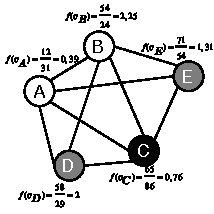
\includegraphics[scale=1.6]{Figures/diag-const-ratio.pdf}
		\caption{\footnotesize Elección de nodo por mayor ratio.}
		\label{fig:const-ratio}
	\end{minipage}
	\hspace{-1cm}
	\begin{minipage}[b]{0.6\linewidth}
		\centering
		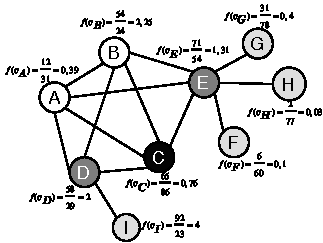
\includegraphics[scale=1.6]{Figures/diag-const-ady.pdf}
		\caption{\footnotesize Elección de nodo por mayor número de adyacentes.}
		\label{fig:const-ady}
	\end{minipage}
\end{figure}
En el caso de la figura \ref{fig:const-ratio} se escoge el nodo $D$ que tiene una relación mayor entre sus pesos $p$ y $q$, $f(v_D)=\frac{58}{29}=2$, respecto del nodo $E$. Como siempre se selecciona un solo nodo en el paso \ref{alg:const_voraz:get_mejor} del algoritmo \ref{alg:const_voraz}, en lugar de un subconjunto de nodos, este caso puede suponer un mayor ratio final.

Por otro lado, en la figura \ref{fig:const-ady}, se observa la opción de escoger el nodo con mayor número de vecinos. A priori, puede suponer una mejor solución añadir mayor cantidad de adyacentes y por lo tanto, mayor ratio. Al tratarse de un algoritmo voraz, esta estrategia puede dejar atrás nodos más prometedores para alcanzar mayor ratio en la solución final. En este ejemplo, se escoge como mejor nodo el $E$, ya que tiene más adyacentes. Posteriormente se añade, por ejemplo, el nodo $G$, obteniendo un ratio de $f(\{v_A,v_B,v_C,v_E,v_G\})=0,96$. Esta selección está dejando atrás los nodos $D$ e $I$, los cuáles aportan mayor ratio a la solución, con un valor en este caso de $f(\{v_A,v_B,v_C,v_D,v_I\})=1,46$, superior al obtenido mediante el otro constructivo.

\subsection{Fase de mejora}
\label{sec:faseBusqueda}
Para esta segunda fase, se ha definido el algoritmo \ref{alg:bl}, el cuál parte de la solución obtenida previamente en la fase constructiva, formada por los nodos que forman un clique.

\begin{algorithm}
	$ vecinos \gets \emptyset $ \\[0.2cm] \label{alg:mj:vecVacios}
	$ vecinos \gets obtenerVecinos(solución)$ \\[0.2cm] \label{alg:mj:getVecSol}
	$ vecinosOrdenados \gets ordenarVecinos(vecinos)$ \\[0.2cm] \label{alg:mj:ordVecs}
	\For{nodo $\epsilon$ vecinosOrdenados}{ \label{alg:mj:for}
		$ solucion \gets incluirNodo(solución, nodo) $ \\[0.2cm] \label{alg:mj:addNodoSol}
		\If{$ no \hspace{0.1cm} esClique(solución) $}{ \label{alg:mj:conNoClique}
			$ solución \gets excluirNodo(solución, nodo) $ \\[0.2cm] \label{alg:mj:exNodo}
		}
		$ solución \gets incluirAdyacentes(solución, nodo) $ \\[0.2cm] \label{alg:mj:addAdys}
	}
	\Return solución \label{alg:mj:rtSol}
	\caption{Pseudocódigo algoritmo búsqueda local.}
	\label{alg:bl}
\end{algorithm}

Con esta solución se obtienen en el paso \ref{alg:mj:getVecSol} todos los vecinos de cada nodo de esta. Estos son ordenados de mayor a menor ratio en el paso \ref{alg:mj:ordVecs}. Esta ordenación se realiza con el fin de aumentar las posibilidades de obtener un mejor valor de ratio. Se obtiene el primer nodo del listado y se añade a la solución, paso \ref{alg:mj:conNoClique}, comprobando posteriormente si esta solución forma o no un nuevo clique en el paso \ref{alg:mj:conNoClique}. Esta comprobación verifica que todos los nodos son adyacentes entre sí, formando un clique.

Si añadir el nodo no formara una solución, en el paso \ref{alg:mj:exNodo} se excluyen todos los nodos que impiden que se forme una solución factible.
En caso contrario, ese nodo añadido en el paso \ref{alg:mj:addNodoSol} se mantendría y a su vez, en el paso \ref{alg:mj:addAdys}, se añadirían todos sus nodos adyacentes, con el fin de obtener un clique de tamaño máximo, como marca la restricción del problema.
Finalmente, una vez comprobados todos los nodos se devuelve el listado solución en el paso \ref{alg:mj:rtSol}.

%-------------------------------------------------------------------------------

